
%%%%%%%%%%%%%%%%%%%%%%% file typeinst.tex %%%%%%%%%%%%%%%%%%%%%%%%%
%
% This is the LaTeX source for the instructions to authors using
% the LaTeX document class 'llncs.cls' for contributions to
% the Lecture Notes in Computer Sciences series.
% http://www.springer.com/lncs       Springer Heidelberg 2006/05/04
%
% It may be used as a template for your own input - copy it
% to a new file with a new name and use it as the basis
% for your article.
%
% NB: the document class 'llncs' has its own and detailed documentation, see
% ftp://ftp.springer.de/data/pubftp/pub/tex/latex/llncs/latex2e/llncsdoc.pdf
%
%%%%%%%%%%%%%%%%%%%%%%%%%%%%%%%%%%%%%%%%%%%%%%%%%%%%%%%%%%%%%%%%%%%


\documentclass[runningheads,a4paper]{llncs}

\usepackage{amssymb}
\setcounter{tocdepth}{3}
\usepackage{graphicx}


\usepackage{rotating, longtable, hhline}
\usepackage{amsmath, amssymb}
\usepackage{amsfonts}
\usepackage{url}
\urldef{\mailsa}\path|{alfred.hofmann, ursula.barth, ingrid.haas, frank.holzwarth,|
\urldef{\mailsb}\path|anna.kramer, leonie.kunz, christine.reiss, nicole.sator,|
\urldef{\mailsc}\path|erika.siebert-cole, peter.strasser, lncs}@springer.com|    
\newcommand{\keywords}[1]{\par\addvspace\baselineskip
\noindent\keywordname\enspace\ignorespaces#1}
\newcommand{\MarkThree}{\{(\Gamma_i, \varkappa_{3,i}); \hm{} i \geqslant 0\}}
\newcommand*{\hm}[1]{#1\nobreak\discretionary{}%
	{\hbox{$\mathsurround=0pt #1$}}{}}% перенос арифметических знаков

\begin{document}

\mainmatter  % start of an individual contribution

% first the title is needed
\title{Low-priority queue and server's steady-state existence in a tandem under prolongable cyclic service}

% a short form should be given in case it is too long for the running head
\titlerunning{Low-priority queue and server's steady-state existence}

% the name(s) of the author(s) follow(s) next
%
% NB: Chinese authors should write their first names(s) in front of
% their surnames. This ensures that the names appear correctly in
% the running heads and the author index.
%
\author{Victor Kocheganov \and Andrei Zorine}
%
\authorrunning{Low-priority Queue in Tandem of Queuing Systems}
% (feature abused for this document to repeat the title also on left hand pages)

% the affiliations are given next; don't give your e-mail address
% unless you accept that it will be published
\institute{Institute of Information Technology, Mathematics and Mechanics\\
N.~I.~Lobachevsky State University of Nizhny Novgorod, \\ Gagarina av. 23, 603950 Nizhni Novgorod, Russia}

%
% NB: a more complex sample for affiliations and the mapping to the
% corresponding authors can be found in the file "llncs.dem"
% (search for the string "\mainmatter" where a contribution starts).
% "llncs.dem" accompanies the document class "llncs.cls".
%

\toctitle{Lecture Notes in Computer Science}
\tocauthor{Authors' Instructions}
\maketitle


\begin{abstract}
A mathematical model of a tandem of queuing systems is considered. Each system has a high-priority input flow and a low-priority input flow which are conflicting. In the first system, the customers are serviced in the class of cyclic algorithms. The serviced high-priority customers are transferred from the first system to the second one  with random delays and become the high-priority input flow of the second system. In the second system, customers are serviced in the class of cyclic algorithms with prolongations. Low-priority customers are serviced when their number exceeds a threshold. A mathematical model is constructed in form of a multidimensional denumerable discrete-time Markov chain. Conditions of low-priority queue stationary distribution existence were found.
\keywords{tandem of controlling queuing systems, cyclic algorithm with prolongations, conflicting flows, multidimensional denumerable dis-crete-time Markov chain}
\end{abstract}


\section{Introduction}
An enormous amount of work has been done on the problem of conflicting traffic flows control at crossroad by the moment. In the queuing theory literature one can find following algorithms investigated: fixed duration cyclic algorithm, cyclic algorithm with a loop, cyclic algorithm with changing regimes, etc~\cite{n:f:p:1968,f:1977,f:1977-1,l:f:2000,p:f:2008,a:b:2010}. However, in a real-life situations cars pass several consecutive crossroads on their way rather then only one. In other words, an output flow of cars from
the first intersection forms an input flow of cars of the next intersection. Hence, the second input flow
no longer has an \textit{a priori} known simple probabilistic structure (for example, a
non-ordinary Poison flow), and knowledge about the service algorithm should be taken into account to deduce formation conditions of the first output flow.

One can find several works about tandems of intersections. In~\cite{y:l:1985} a computer-aided
simulation of adjacent intersections was carried out. In~\cite{z:2012} a mathematical model of two intersections in tandem governed by cyclic algorithms was investigated and stability conditions were found. In this paper we assume that the first intersection is governed by a cyclic algorithm while the second intersection is governed by a cyclic algorithm with prolongations. The low-priority queue on the second intersection and necessary conditions of its stationary state existence take central place of this paper. This work continues studying in paper \cite{k:z:2016}.

\section{The  problem settings}

Consider a queuing system with a scheme shown in Fig.~\ref{SystemScheme}.  
\begin{figure}[h!]
   \centering
    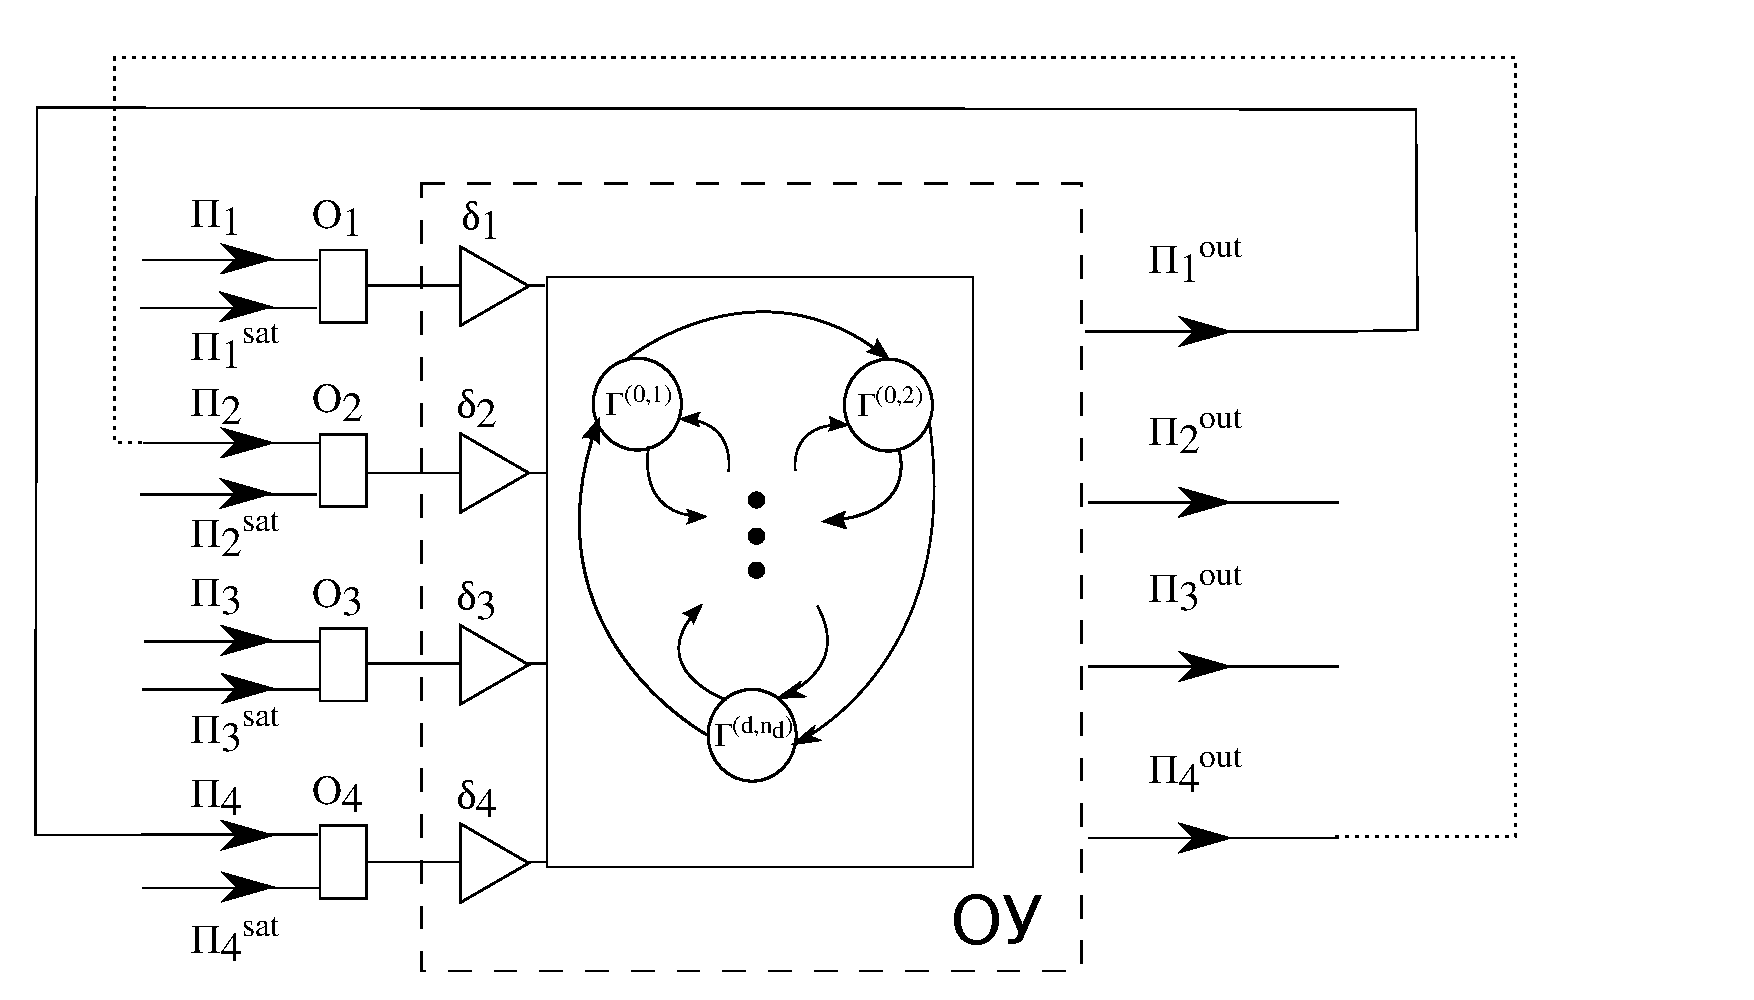
\includegraphics[width=\textwidth]{SystemScheme.pdf} % or {1.eps} in case of EPS format of the picture
    \caption {Scheme of the queuing system as a cybernetic control system}
    \label{SystemScheme}
\end{figure}
There are four
input flows of customers $\Pi_1$, $\Pi_2$, $\Pi_3$, and $\Pi_4$ entering the single server queueing
system. Customers in the input flow $\Pi_j$, $j \in \{1,2,3,4\}$ join a queue $O_j$ with an
unlimited capacity. For $j \in \{1,2,3\}$ the discipline of the queue $O_j$ is FIFO (First In First
Out). Discipline of the queue $O_4$ will be described later. The input flows $\Pi_1$ and $\Pi_3$ are
generated by an external environment, which has only one state. Each of these flows is a nonordinary
Poisson flow. Denote by $\lambda_1$ and $\lambda_3$ the intensities of bulk arrivals for the flows
$\Pi_1$ and $\Pi_3$ respectively. The probability generating function of number of customers in a
bulk in the flow $\Pi_j$ is
\begin{equation}
f_j(z) = \sum_{\nu=1}^{\infty} p_{\nu}^{(j)} z ^{\nu}, \quad j\in \{1,3\}.
\label{GeneratingFunc}
\end{equation}
We assume that $f_j(z)$ converges for any $z\in \mathbb{C}$ such that $|z|<(1+\varepsilon)$,
$\varepsilon>0$. Here $p_{\nu}^{(j)}$ is the probability of a bulk size in flow $\Pi_j$ being
exactly $\nu=1$, $2$, \ldots. Having been serviced the customers from $O_1$ come back to the system
as the $\Pi_4$ customers. The $\Pi_4$ customers in turn after service enter the system as the
$\Pi_2$ ones. The flows $\Pi_2$ and $\Pi_3$ are conflicting in the sense that their customers can't
be serviced simultaneously. This implies that the problem can't be reduced to a problem with fewer
input flows by merging the flows together.


In order to describe the server behavior we fix positive integers $d$, $n_0$, $n_1$, $\ldots$,
$n_d$ and we introduce a finite set $\Gamma=\{\Gamma^{(k,r)} \colon k=0,1,\ldots,d; r=1,2,\ldots
n_k\}$ of states server can reside in. At the state $\Gamma^{(k,r)}$ the server stays during a constant 
time $T^{(k,r)}$. Define disjoint subsets $\Gamma^{\mathrm{I}}$, $\Gamma^{\mathrm{II}}$,
$\Gamma^{\mathrm{III}}$, and $\Gamma^{\mathrm{IV}}$ of $\Gamma$ as follows.  In the state $\gamma
\in \Gamma^{\mathrm{I}}$ only customers from the queues $O_1$, $O_2$ and $O_4$ are serviced.  In the
state $\gamma \in \Gamma^{\mathrm{II}}$ only customers from the queues $O_2$ and $O_4$ are serviced.
In the state $\gamma \in \Gamma^{\mathrm{III}}$ only customers from queues $O_1$, $O_3$, and $O_4$
are serviced.  In the state $\gamma \in \Gamma^{\mathrm{IV}}$ only customers from queues $O_3$ and
$O_4$ are serviced.  We assume that $\Gamma = \Gamma^{\mathrm{I}} \cup \Gamma^{\mathrm{II}} \cup
\Gamma^{\mathrm{III}} \cup \Gamma^{\mathrm{IV}}$. Set also ${}^1\Gamma=\Gamma^{\mathrm{I}} \cup
\Gamma^{\mathrm{III}}$, ${}^2\Gamma=\Gamma^{\mathrm{I}} \cup \Gamma^{\mathrm{II}}$,
${}^3\Gamma=\Gamma^{\mathrm{III}} \cup \Gamma^{\mathrm{IV}}$.

The server changes its state according to the following rules. We call a set $C_k = \{\Gamma^{(k,r)}
\colon r=1,2,\ldots n_k\}$ the $k$-th cycle, $k=1$, $2$, $\ldots$, $d$. For $k=0$ the state
$\Gamma^{(0,r)}$ with $r=1$, $2$, $\ldots$, $n_0$ is called a prolongation state. Put $r \oplus_k 1
= r+1$ for $r<n_k$, and $r \oplus_k 1 = 1$ for $r=n_k$ ($k = 0$, $1$, $\ldots$, $d$). In the cycle
$C_k$ we select a subset $C_k^{\mathrm{O}}$ of input states, a subset $C_k^{\mathrm{I}}$ of output
states, and a subset $C_k^{\mathrm{N}} = C_k \setminus (C_k^{\mathrm{O}} \cup C_k^{\mathrm{I}})$ of
neutral states.  After the state $\Gamma^{(k,r)} \in C_k\setminus C_k^{\mathrm{O}}$ the server
switches to the state $\Gamma^{(k,r \oplus_k 1)}$ within the same cycle $C_k$.  After the state
$\Gamma^{(k,r)}$ in $C_k^{\mathrm{O}}$ the server switches to the state $\Gamma^{(k,r \oplus_k 1)}$
if number of customers in the queue $O_3$ at switching instant is greater than a predetermined
threshold $L$.  Otherwise, if the number of customers in the queue $O_3$ is less than or equal to $L$
then the new state is the prolongation one $\Gamma^{(0,r_1)}$ where $r_1=h_1(\Gamma^{(k,r)})$ and
$h_1(\cdot)$ is a given mapping of $\bigcup_{k=1}^d C_k^{\mathrm{O}}$ into $\{1,2,\ldots,
n_0\}$.  After the state $\Gamma^{(0,r)}$ if the number of customers in $O_3$ is not above $L$ the
state of the same type $\Gamma^{(0,r_2)}$ is chosen where $r_2=h_2(r)$ and $h_2(\cdot)$ is a given
mapping of the set $\{1,2, \ldots, n_0\}$ into itself; in the other case the new state is
$\Gamma^{(k,r_3)} \in C_k^{\mathrm{I}}$ where $\Gamma^{(k,r_3)}=h_3(r)$ and $h_3(\cdot)$ is a 
given mapping of  $\{1,2, \ldots, n_0\}$ to $\bigcup_{k=1}^d C_k^{\mathrm{I}}$. We assume
that each prolongation state $\Gamma^{(0,r)}$ belongs to the set ${}^2 \Gamma$ and that relations
$C_k^\mathrm{O}\subset {}^2 \Gamma$ and $C_k^\mathrm{I}\subset {}^3 \Gamma$ hold. We also assume
that all the cycles have exactly one input and output state. Finally, we assume that all the
prolongation states make a cycle, that is  $h_2(r)=r\oplus_0 1$. Putting all together, we introduce
a function which formalizes the server state changes:
\begin{equation}
h(\Gamma^{(k,r)},y) = 
\begin{cases}
\Gamma^{(k,r \oplus_k 1)}&  \text{ if  $\Gamma^{(k,r)}\in C_k\setminus C_k^{\mathrm{O}}$ or} \\ & \quad \text{$(\Gamma^{(k,r)}\in C_k^{\mathrm{O}}) \wedge (y>L)$;}\\
\Gamma^{(0,h_1(\Gamma^{(k,r)}))}&  \text{ if  $\Gamma^{(k,r)}\in C_k^{\mathrm{O}}$ and $y\leqslant L$;}\\
\Gamma^{(0,r \oplus_0 1)}&  \text{ if $k=0$ and $y\leqslant L$;}\\
h_3(r)&  \text{ if  $k=0$ and $y > L$.}
\end{cases}
\label{hLaw}
\end{equation}


In general, service durations of different customers can be dependent and may have different laws of
probability distributions. So, saturation flows will be used to define the service process. A
saturation flow $\Pi^{\mathrm{\text{sat}}}_j$, $j \in \{1,2,3,4\}$, is defined as a virtual output
flow under the maximum usage of the server and unlimited number of customer in the queue $O_j$. The
saturation flow $\Pi^{\mathrm{\text{sat}}}_j$, $j\in \{1,2,3\}$ contains a non-random number
$\ell({k,r,j)}\geqslant0$ of customers in the server state $\Gamma^{(k,r)}$. In particular,
$\ell({k,r,j)}\geqslant1$ for $\Gamma^{(k,r)}\in{}^j\Gamma$ and $\ell({k,r,j)}=0$ for
$\Gamma^{(k,r)}\not\in{}^j\Gamma$. Let $\mathbb{Z}_+$ be
the set of non-negative integer numbers. If the queue $O_4$ contains $x \in \mathbb{Z}_+$ customers
the saturation flow $\Pi^{\mathrm{\text{sat}}}_4$ also contains the $x$ customers.  Finally, in the
state $\Gamma^{(k,r)}$ every customer from queue $O_4$ with probability $p_{k,r}$ and independently
of others ends servicing and joins $\Pi_2$ to go to $O_2$. With the complementary probability
$1-p_{k,r}$ the customer stays in $O_4$ until the next time slot. In the next time slot it repeats
its attempt to join $\Pi_2$ with a proper probability.

A real-life example of just described queuing system is a tandem of two consecutive crossroads
(Fig. \ref{crossroads}).
\begin{figure}[h!]
   \centering
    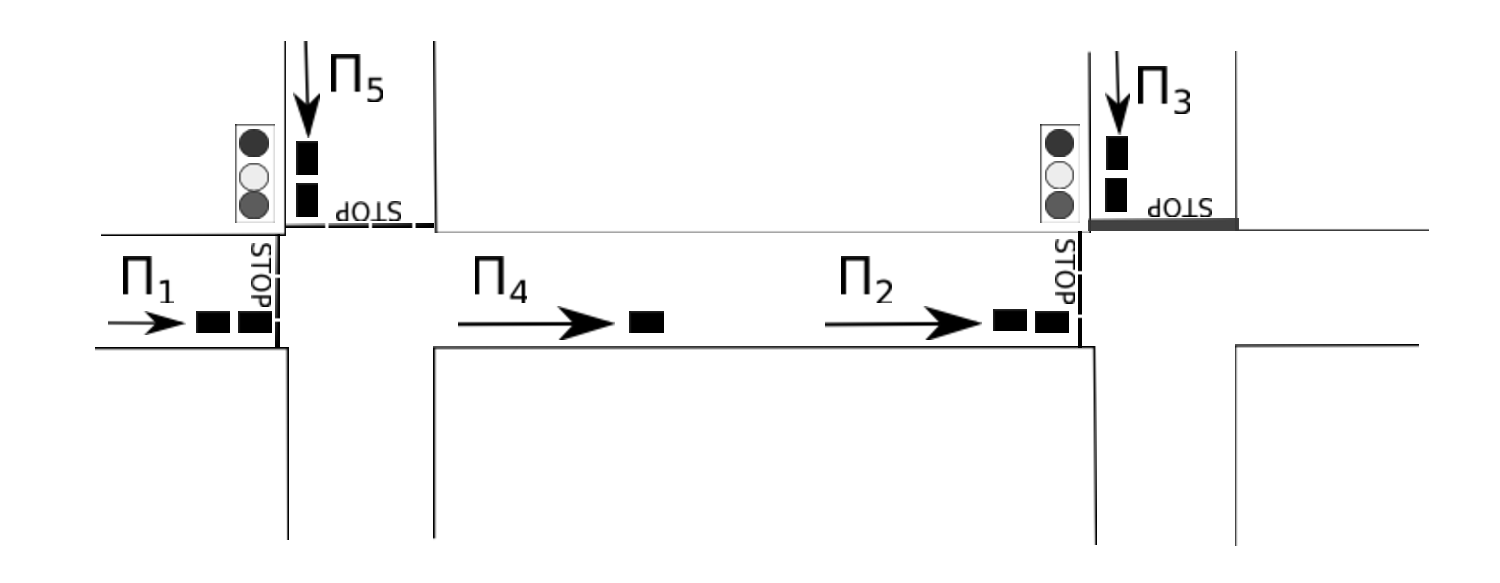
\includegraphics[width=\textwidth]{Crossroads.pdf} 
    \caption {A tandem of crossroads, the physical interpretation of the queuing system under study}
    \label{crossroads}
\end{figure}
The input flows are flows of vehicles. The flows $\Pi_1$ and $\Pi_5$ at the first crossroad are
conflicting; $\Pi_2$ and $\Pi_3$ at the second crossroad are also conflicting. Every vehicle from
the flow $\Pi_1$ after passing first road intersection joint the flow $\Pi_4$ and enters the queue
$O_4$. After some random time interval the vehicle arrives to the next road intersection. Such a pair
of crossroads is an instance of a more general queuing model described above.

\section{Mathematical model}
The queuing system under investigation can be regarded as a cybernetic control system that helps to
rigorously construct a formal stochastic model~\cite{z:2012}. The scheme of the control system is
shown in Fig.~\ref{SystemScheme}. There are following blocks present in the scheme: 1)~the external
environment with one state; 2) input poles of the first type~--- the input flows $\Pi_1$, $\Pi_2$,
$\Pi_3$, and $\Pi_4$; 3) input poles of the second type~--- the saturation flows
$\Pi^{\mathrm{\text{sat}}}_1$, $\Pi^{\mathrm{\text{sat}}}_2$, $\Pi^{\mathrm{\text{sat}}}_3$, and
$\Pi^{\mathrm{\text{sat}}}_4$; 4)~an external memory~--- the queues $O_1$, $O_2$, $O_3$, and $O_4$;
5)~an information processing device for the external memory~--- the queue discipline units
$\delta_1$, $\delta_2$, $\delta_3$, and $\delta_4$; 6) an internal memory --- the server (OY); 7)~an
information processing device for internal memory~--- the graph of server state transitions;
8)~output poles~--- the output flows $\Pi^{\mathrm{\text{out}}}_1$, $\Pi^{\mathrm{\text{out}}}_2$,
$\Pi^{\mathrm{\text{out}}}_3$, and $\Pi^{\mathrm{\text{out}}}_4$.  The coordinate of a block is
its number on the scheme.

Let us  introduce the following variables and elements along with their
value ranges. To fix a discrete time scale consider the epochs $\tau_0=0$, $\tau_1$, $\tau_2$,
$\ldots$ when the server changes its state. Let $\Gamma_i\in\Gamma$ be the server state
during the interval $(\tau_{i-1};\tau_i]$, $\varkappa_{j,i} \in \mathbb{Z}_+ $ be the number of customers in
the queue $O_j$ at the instant $\tau_i$, $\eta_{j,i} \in \mathbb{Z}_+$ be the number of customers
arrived into the queue $O_j$ from the flow $\Pi_j$ during the interval $(\tau_{i};\tau_{i+1}]$, $\xi_{j,i} \in
\mathbb{Z}_+$ be the number of customers in the saturation flow $\Pi^{\mathrm{\text{sat}}}_j$ during
the interval $(\tau_{i};\tau_{i+1}]$, $\overline{\xi}_{j,i}\in \mathbb{Z}_+$ be the actual number of 
serviced customers from the queue  $O_j$ during the interval $(\tau_{i};\tau_{i+1}]$, $j\in
\{1,2,3,4\}$.

The server changes its state according to the following rule:
\begin{equation}
\Gamma_{i+1}=h(\Gamma_i,\varkappa_{3,i})
\label{gammaFunc}
\end{equation}
where the mapping $h(\cdot,\cdot)$ is defined by Formula~\eqref{hLaw}.

Let $\varphi_1(\cdot,\cdot)$ and $\varphi_3(\cdot,\cdot)$ be defined by series expansions
\begin{equation*}
\sum_{\nu=0}^{\infty} z^\nu\varphi_j(\nu,t) = \exp\{\lambda_j t (f_j(z)-1)\}
\end{equation*}
with functions $f_j(z)$ defined by \eqref{GeneratingFunc}, $j \in \{1,3\}$. The function
$\varphi_j(\nu,t)$ equals the probability of  $\nu=0$, $1$, $\ldots${} arrivals in the flow
$\Pi_j$ during time $t \geqslant 0$. If $\nu < 0$ the value of $\varphi_j(\nu,t)$ is set to
zero.

Mathematical model in more details can be found in work \cite{k:z:2016}. From now on we focus on low-priority customers in the queue $O_3$. 

\section{The low-priority queue}
Here we will consider the stochastic sequence
\begin{equation}
\label{eq:theMC}
\{(\Gamma_i(\omega), \varkappa_{3, i}(\omega)); i =0, 1, \ldots\},
\end{equation}
which includes the number of low-priority customers $\varkappa_{3, i}(\omega)$ in the queue $O_3$.  In this
section we will report several results concerning this stochastic sequence.

Let $\Gamma^{(k,r)}\in \Gamma$ and $x_3 \in Z_+$. Denote by 
$H_{-1}(\Gamma^{(k,r)}, x_3)$ the set of all server states $\gamma$ such that $h(\gamma, x_3) =
\Gamma^{(k,r)}$ and put $r \ominus_k 1
= r-1$ for $n_k \geqslant r>1$, and $r \ominus_k 1 = n_k$ for $r=1$ ($k = 0$, $1$, $\ldots$, $d$).
Then formula \eqref{hLaw} makes it possible to define  the mapping $H_{-1}(\Gamma^{(k,r)}, x_3)$ explicitly:
\begin{equation}
H_{-1}(\Gamma^{(k,r)}, x_3) = 
\begin{cases}
\bigl\{\Gamma^{(k_1,r_1)}, \Gamma^{(0,r\ominus_0 1)}\bigr\}&  \text{ if  $(k=0) \wedge (x_3 \leqslant L)$,}\\
\bigl\{\Gamma^{(k,r\ominus_k 1)}, \Gamma^{(0,r_2)}\bigr\}&  \text{ if  $(\Gamma^{(k,r)}\in C_k^{\mathrm{I}})
  \wedge (x_3>L)$,}\\ 
\bigl\{\Gamma^{(k,r\ominus_k 1)}\bigr\}&  \text{ if  $(\Gamma^{(k,r)}\in C_k^{\mathrm{O}}) \vee (\Gamma^{(k,r)}\in C_k^{\mathrm{N}})$;}\\
\varnothing&  \text{ if  $(k = 0)\wedge  (x_3>L)$}\\
 & \qquad \text{ or $(\Gamma^{(k,r)}\in C_k^{\mathrm{I}}) \wedge (x_3\leqslant L)$}
\end{cases}
\end{equation}
where $h_1(\Gamma^{(k_1,r_1)})=r$ and $h_3(r_2)=\Gamma^{(k,r)}$.

Let's define for $\gamma \in \Gamma$ and $x_3 \in Z_+$ values
\begin{equation*}
Q_{3,i}(\gamma,x) = {\mathbf P}(\{\omega\colon \Gamma_{i}(\omega)=\gamma, \varkappa_{3,i}(\omega)=x_3\}).
\end{equation*}

Theorem~\ref{theorem:gen} concerns generating functions and corrects ones in paper \cite{k:z:2016}. Suppose $k$ and $r$ are such that $\Gamma^{(k,r)}\in \Gamma$. Let's define  partial probability generating functions 
\begin{align*}
&\mathfrak{M}^{(3,i)}(k,r,v) = \sum_{w=0}^{\infty} Q_{3,i}(\Gamma^{(k,r)},w) v^w,\\
&q_{k,r}(v) = v^{-\ell(k,r,3)}\sum_{w=0}^{\infty} \varphi_3(w,T^{(k,r)})v^w.
\end{align*}
%\begin{equation*}
%\mathfrak{M}^{(i)}(k,r,v) = \sum_{w=0}^{\infty} Q_{3,i}(\Gamma^{(k,r)},w) v^w,
%q_{k,r}(v) = v^{-\ell(k,r,3)}\sum_{w=0}^{\infty} \varphi_3(w,T^{(k,r)})v^w.
%\end{equation*}
and auxilary functions
\begin{multline*}
\tilde{\alpha}_i(k,r,v) = \sum_{x_3=0}^{\ell(k,r,3)}\sum_{\gamma \in H_{-1}(\tilde{\gamma},x_3)} Q_{3,i}(\gamma,x_3) \sum_{a=0}^{\ell(k,r,3) - x_3} \varphi_3(a,T^{(k,r)}) - \\
- \sum_{x_3=0}^{\ell(k,r,3)}  \sum_{\gamma \in H_{-1}(\tilde{\gamma},x_3)} Q_{3,i}(\gamma,x_3) v^{x_3-\ell(k,r,3)}  \sum_{w=0}^{\ell(k,r,3) -x_3}
\varphi_3(w,T^{(k,r)}) v^w,
\end{multline*}
\begin{multline*}
\alpha_i(0,r,v) =\tilde{\alpha}_i(0,r,v) + q_{0,r}(v) \times \sum_{x_3=0}^{L} \left[ Q_{3,i}(\Gamma^{(k_1,r_1)},x_3) +\right. \\
\left. + Q_{3,i}(\Gamma^{(0,r\ominus_0 1)},x_3) \right] v^{x_3}, \quad \Gamma^{(0,r)} \in \Gamma,
\end{multline*}
\begin{multline*}
\alpha_i(k,r,v) =\tilde{\alpha}_i(k,r,v) - q_{k,r}(v)\sum_{x_3=0}^{L} \left[ Q_{3,i}(\Gamma^{(k,r\ominus_{k} 1)},x_3) \right. + \\ +\left.  Q_{3,i}(\Gamma^{(0,r_2)},x_3) \right] v^{x_3}
+ q_{k,r}(v)\sum_{x_3 \geqslant 0} Q_{3,i}(\Gamma^{(0,r)},x_3)v^{x_3}, \quad \Gamma^{(k, r)} \in C_{k}^{\mathrm{I}},
\end{multline*}
\begin{equation*}
\alpha_i(k,r,v) =\tilde{\alpha}_i(k,r,v), \quad \Gamma^{(k, r)} \in C_{k}^{\mathrm{O}} \cup C_{k}^{\mathrm{N}}.
\end{equation*}
\begin{theorem}
Following recurrent w.r.t. $i
\geqslant 0$ relations take place for the  partial probability generating functions:
\begin{enumerate}
\item $\Gamma^{(0,r)} \in \Gamma$, $r = \overline{1,n_0}$ 
$$
\mathfrak{M}^{(3,i+1)}(0,r,v) = \alpha_i(0,r,v);
$$
\item $\Gamma^{(k,r)} \in \Gamma $, $k =\overline{1,d}$, $r=\overline{1,n_{k}}$
$$
\mathfrak{M}^{(3,i+1)}(k,r,v) = q_{k,r} (v)\times  \mathfrak{M}^{(3,i)}(k,r \ominus_{k} 1,v) + \alpha_i(k,r,v);
$$
\end{enumerate}
\label{theorem:gen}
\end{theorem}


The last result (theorem \ref{theorem:nec}) is new and concerns low-priority queue and server's steady-state existence.
\begin{theorem}
For Markov chain~\eqref{eq:theMC} to have stationary distribution $Q_3(\gamma,x)$, $(\gamma,x)\in \Gamma \times {\mathbb Z}_+$ it is necessary that  following inequality takes place
$$
\min_{k=\overline{1,d}} { \frac{\lambda_3 f_3'(1) \sum_{r = 1}^{n_k} T^{(k,r)}}  {\sum_{r = 1}^{n_{k}}\ell(k,r,3)}} <1.
$$
\label{theorem:nec}
\end{theorem}


\begin{proof}

Let's assume that stationary distribution $Q_3(\gamma,x)$, $(\gamma,x)\in \Gamma \times {\mathbb Z}_+$, 
exists. Then choosing this distribution as the  initial one imposes existence of following limits:
$$
\lim_{i\to \infty} Q_{3,i}(\gamma,w) = Q_3(\gamma,w),
$$
which are equal to stationary probabilities of corresponding states.

After defining generating functions
$$
\mathfrak{M}^{(3)}(k,r,v) = \sum_{w=0}^{\infty} Q_3(\gamma,w) v^w,
$$
 for the stationary distribution similar relations can be derived as in Theorem~1:
 \begin{enumerate}
\item $ \Gamma^{(0,r)} \in \Gamma$, $r = \overline{1,n_0}$ 
\begin{equation}
\mathfrak{M}^{(3)}(0,r,v) = \alpha(0,r,v);
\label{three:generation:one}
\end{equation}
\item $\Gamma^{(k,r)} \in \Gamma $, $k =\overline{1,d}$, $r=\overline{1,n_k}$
\begin{equation}
\mathfrak{M}^{(3)}(k,r,v) = q_{k,r} (v)\times  \mathfrak{M}^{(3)}(k,r \ominus_{k} 1,v) + \alpha(k,r,v);
\label{three:generation:two}
\end{equation}
\end{enumerate}
where 
\begin{multline*}
\tilde{\alpha}(k,r,v) = \sum_{x_3=0}^{\ell(k,r,3)}\sum_{\gamma \in {\mathbb H}_{-1}(\tilde{\gamma},x_3)} Q_3(\gamma,x_3) \sum_{a=0}^{\ell(k,r,3) - x_3} \varphi_3(a,T^{(k,r)}) - \\
- \sum_{x_3=0}^{\ell(k,r,3)}  \sum_{\gamma \in {\mathbb H}_{-1}(\tilde{\gamma},x_3)} Q_3(\gamma,x_3)v^{x_3-\ell(k,r,3)} \sum_{w=0}^{\ell(k,r,3) -x_3}
\varphi_3(w,T^{(k,r)}) v^w,
\end{multline*}
\begin{multline*}
\alpha(0,r,v) =\tilde{\alpha}(0,r,v) + q_{0,r}(v) \times \sum_{x_3=0}^{L} \left[ Q_{3}(\Gamma^{(k_1,r_1)},x_3) +\right. \\
\left. + Q_{3}(\Gamma^{(0,r\ominus_0 1)},x_3) \right] v^{x_3}, \quad \Gamma^{(0,r)} \in \Gamma,
\end{multline*}
\begin{multline*}
\alpha(k,r,v) =\tilde{\alpha}(k,r,v) - q_{k,r}(v)\sum_{x_3=0}^{L} \left[ Q_{3}(\Gamma^{(k,r\ominus_{k} 1)},x_3) \right. + \\ +\left.  Q_{3}(\Gamma^{(0,r_2)},x_3) \right] v^{x_3}
+ q_{k,r}(v)\sum_{x_3 \geqslant 0} Q_{3}(\Gamma^{(0,r)},x_3)v^{x_3}, \quad \Gamma^{(k, r)} \in C_{k}^{\mathrm{I}},
\end{multline*}
\begin{equation*}
\alpha(k,r,v) =\tilde{\alpha}(k,r,v), \quad \Gamma^{(k, r)} \in C_{k}^{\mathrm{O}} \cup C_{k}^{\mathrm{N}}
\end{equation*}

Taylor expansion of $q_{k,r}(v)$ gives 
\begin{multline*}
    q_{k,r}(v) =  v^{-\ell(k,r,3)} \exp{(\lambda_3 T^{(k,r)} (f_3(v)-1))}= \\=1 + (\lambda_3 T^{(k,r)} f_3'(1) - \ell(k,r,3))(v-1) + O((v-1)^2)).
\end{multline*}

Summing all the relations \eqref{three:generation:one} and \eqref{three:generation:two} one can find
\begin{multline}
 \sum_{k=0}^{d} \sum_{r=1}^{n_k} \mathfrak{M}^{(3)}(k,r,v) =\\
 =\sum_{r=1}^{n_0} \alpha (0,r,v) + \sum_{k=1}^{d}\sum_{r=1}^{n_k} \bigl[ q_{k,r}(v) \mathfrak{M}^{(3)}(k,r\ominus_k 1,v) + \alpha(k,r,v)\bigr] = \\
 = \sum_{k=1}^{d}\sum_{r=1}^{n_k} q_{k,r}(v) \mathfrak{M}^{(3)}(k,r\ominus_k 1,v)   + \sum_{k=1}^{d}\sum_{r=1}^{n_k} \alpha(k,r,v)  + \sum_{r=1}^{n_0} \alpha (0,r,v).
 \label{summed:neccessary}
\end{multline}

Similarly lets expand $\sum_{k=1}^{d}\sum_{r=1}^{n_k} \alpha(k,r,v)$ and $\sum_{r=1}^{n_0} \alpha (0,r,v)$. First of all
\begin{multline*}
    \tilde{\alpha} (k,r,v) =\\
    = \sum_{x_3=0}^{\ell(k,r,3)}\sum_{\gamma \in {\mathbb H}_{-1}(\tilde{\gamma},x_3)} Q_3(\gamma,x_3) \sum_{w=0}^{\ell(k,r,3) - x_3} \varphi_3(w,T^{(k,r)}) (1-v^{w-(\ell(k,r,3)-x_3)})=\\= - (v-1) \sum_{x_3=0}^{\ell(k,r,3)}\sum_{\gamma \in {\mathbb H}_{-1}(\tilde{\gamma},x_3)} Q_3(\gamma,x_3) \times \\
    \times \sum_{w=0}^{\ell(k,r,3) - x_3} \varphi_3(w,T^{(k,r)}) (w-(\ell(k,r,3)-x_3)) + O((v-1)^2).
\end{multline*}
In particular, $\ell(k,r,3)$ equals to zero for $k=0$, that implies $\tilde{\alpha} (0,r,v) \hm= O((v\hm-1)^2)$.

And now we are ready to expand further:
\begin{multline*}
    \sum_{r=1}^{n_0} \alpha (0,r,v) = \\
    =\sum_{r=1}^{n_0} q_{0,r}(v) \times \sum_{x_3=0}^{L} \bigl[ Q_3(\Gamma^{(k_1,r_1)},x_3) + Q_3(\Gamma^{(0,r\ominus_0 1)},x_3) \bigr] v^{x_3} + O((v-1)^2) =\\
    = \sum_{r=1}^{n_0}(1 + (\lambda_3 T^{(0,r)} f_3'(1) - \ell(0,r,3))(v-1))  \times  \\
    \times \sum_{x_3=0}^{L} \left[ Q_3(\Gamma^{(k_1,r_1)},x_3) + Q_3(\Gamma^{(0,r\ominus_0 1)},x_3) \right] v^{x_3} + O((v-1)^2),
\end{multline*}
\begin{multline*}
    \sum_{k,r\colon \Gamma^{(k, r)} \in C_{k}^{\mathrm{I}}} \alpha(k,r,v) =  \sum_{k,r\colon \Gamma^{(k, r)} \in C_{k}^{\mathrm{I}}}q_{k,r}(v) \biggl[ \mathfrak{M}^{(3)}(0,r_2,v) - \\ -   \sum_{x_3=0}^L\bigl(Q_3(\Gamma^{(k,r\ominus_{k} 1)},x_3) + Q_3(\Gamma^{(0,r_2)},x_3) \bigr) v^{x_3} \biggr] + \\ 
    + \sum_{k,r\colon \Gamma^{(k, r)} \in C_{k}^{\mathrm{I}}} \tilde{\alpha}(k,r,v)
    = \sum_{k,r\colon \Gamma^{(k, r)} \in C_{k}^{\mathrm{I}}}(1 + (\lambda_3 T^{(k,r)} f_3'(1) - \ell(k,r,3))(v-1) )\times \\ 
     \times \biggl[ \mathfrak{M}^{(3)}(0,r_2,v) -   \sum_{x_3=0}^L\bigl(Q_3(\Gamma^{(k,r\ominus_{k} 1)},x_3) + Q_3(\Gamma^{(0,r_2)},x_3) \bigr) v^{x_3} \biggr] -\\- (v-1)\sum_{k,r\colon \Gamma^{(k, r)} \in C_{k}^{\mathrm{I}}} \sum_{x_3=0}^{\ell(k,r,3)}\sum_{\gamma \in {\mathbb H}_{-1}(\tilde{\gamma},x_3)} Q_3(\gamma,x_3) \times \\
     \times \sum_{w=0}^{\ell(k,r,3) - x_3} \varphi_3(w,T^{(k,r)}) (w-(\ell(k,r,3)-x_3)) + O((v-1)^2),
 \end{multline*}

\begin{multline*}
    \sum_{k,r\colon \Gamma^{(k, r)} \in C_{k}^{\mathrm{O}}\cup C_{k}^{\mathrm{N}}} \alpha(k,r,v) =  \sum_{k,r\colon \Gamma^{(k, r)} \in C_{k}^{\mathrm{O}}\cup C_{k}^{\mathrm{N}}} \tilde{\alpha}(k,r,v) = \\=
    -(v-1)\sum_{k,r\colon \Gamma^{(k, r)} \in C_{k}^{\mathrm{O}}\cup C_{k}^{\mathrm{N}}} \sum_{x_3=0}^{\ell(k,r,3)}\sum_{\gamma \in {\mathbb H}_{-1}(\tilde{\gamma},x_3)} Q_3(\gamma,x_3) \times \\
    \times \sum_{w=0}^{\ell(k,r,3) - x_3} \varphi_3(w,T^{(k,r)}) (w-(\ell(k,r,3)-x_3))  +O((v-1)^2).
\end{multline*}

It's important to mention, that any input system state corresponds to one and only one prolongation system state. That is why substitution of calculated expressions into \eqref{summed:neccessary} gives:
\begin{multline}
 0 = O((v-1)^2) + (v-1) \sum_{k=1}^{d}\sum_{r=1}^{n_{k}} (\lambda_3 T^{(k,r)} f_3'(1) - \ell(k,r,3)) \mathfrak{M}^{(3)}(k,r\ominus_{k} 1,v)   +\\+  (v-1) \sum_{r=1}^{n_0} (\lambda_3 T^{(0,r)} f_3'(1) - \ell(0,r,3))  \times \sum_{x_3=0}^{L} \left[ Q_3(\Gamma^{(k_1,r_1)},x_3) \right. +\\ \left. + Q_3(\Gamma^{(0,r\ominus_0 1)},x_3) \right] v^{x_3}  + (v-1) \sum_{k,r\colon \Gamma^{(k, r)} \in C_{k}^{\mathrm{I}}} (\lambda_3 T^{(k,r)} f_3'(1) - \ell(k,r,3))\times \\ 
     \times \biggl[ \mathfrak{M}^{(3)}(0,r_2,v) -   \sum_{x_3=0}^L\bigl(Q_3(\Gamma^{(k,r\ominus_{k} 1)},x_3) + Q_3(\Gamma^{(0,r_2)},x_3) \bigr) v^{x_3} \biggr] -\\- (v-1)\sum_{k,r\colon \Gamma^{(k, r)} \in C_{k}^{\mathrm{O}}\cup C_{k}^{\mathrm{N}}} \sum_{x_3=0}^{\ell(k,r,3)}\sum_{\gamma \in {\mathbb H}_{-1}(\tilde{\gamma},x_3)} \bigg(Q_3(\gamma,x_3) \times \\ \times \sum_{w=0}^{\ell(k,r,3) - x_3} \varphi_3(w,T^{(k,r)}) (w-(\ell(k,r,3)-x_3)) \bigg),
\end{multline}
dividing by $(v-1)$ and then sending $v$ to $1$ from the left one continues
\begin{multline}
 0 = \sum_{k,r\colon \Gamma^{(k, r)} \in C_{k}^{\mathrm{I}}} (\lambda_3 T^{(k,r)} f_3'(1) - \ell(k,r,3))
     \times \biggl[\mathfrak{M}^{(3)}(k,r\ominus_{k} 1,1) - \\ - \sum_{x_3=0}^L Q_3(\Gamma^{(k,r\ominus_{k} 1)},x_3)   +  \mathfrak{M}^{(3)}(0,r_2,1) -   \sum_{x_3=0}^L  Q_3(\Gamma^{(0,r_2)},x_3)  \biggr]
 +\\+ \sum_{k,r\colon \Gamma^{(k, r)} \in C_{k}^{\mathrm{O}}\cup C_{k}^{\mathrm{N}}} (\lambda_3 T^{(k,r)} f_3'(1) - \ell(k,r,3)) \mathfrak{M}^{(3)}(k,r\ominus_{k} 1,1)   +\\+ \sum_{r=1}^{n_0} \lambda_3 T^{(0,r)} f_3'(1)  \times \sum_{x_3=0}^{L} \left[ Q_3(\Gamma^{(k_1,r_1)},x_3) + Q_3(\Gamma^{(0,r\ominus_0 1)},x_3) \right]   +\\+  \sum_{k=1}^{d}\sum_{r=1}^{n_{k}} \sum_{x_3=0}^{\ell(k,r,3)}\!\!\sum_{\gamma \in {\mathbb H}_{-1}(\tilde{\gamma},x_3)} \!\!\!Q_3(\gamma,x_3) \!\!\!\!\sum_{w=0}^{\ell(k,r,3) - x_3} \!\!\!\!\!\!\varphi_3(w,T^{(k,r)}) (\ell(k,r,3)-x_3 - w).
 \label{neccessary:to:paste}
\end{multline}

Fixing $v=1$ in corresponding generating functions relations one can get
\begin{align*}
    \mathfrak{M}^{(3)}(0,r,1) &= \sum_{x_3=0}^{L} \biggl(Q_3(\Gamma^{(k_1,r_1)}, x_3) + Q_3(\Gamma^{(0,r\ominus_{0}1)}, x_3) \biggr),\\
    \mathfrak{M}^{(3)}(k,r,1) &=\mathfrak{M}^{(3)}(k,r\ominus_{k}1,1) +\mathfrak{M}^{(3)}(0,r_2,1)-\\
    &\quad\quad\quad -\sum_{x_3=0}^{L} \biggl(Q_3(\Gamma^{(k,r\ominus_{k}1)}, x_3) + Q_3(\Gamma^{(0,r_2)}, x_3) \biggr), \quad  \Gamma^{(k, r)} \in C_{k}^{\mathrm{I}},\displaybreak\\
    \mathfrak{M}^{(3)}(k,r,1) &= \mathfrak{M}^{(3)}(k,r\ominus_k 1,1), \quad \Gamma^{(k, r)} \in C_{k}^{\mathrm{O}} \bigcup C_{k}^{\mathrm{N}}.
\end{align*}
The last equation gives $ \mathfrak{M}^{(3)}(k,n_k,1) =  \mathfrak{M}^{(3)}(k,n_k\ominus_k 1,1) = \ldots =  \mathfrak{M}^{(3)}(k,1,1) = M_k$. Using these facts, let's simplify  expression \eqref{neccessary:to:paste}
\begin{multline*}
 0 = \sum_{k,r\colon \Gamma^{(k, r)} \in C_{k}^{\mathrm{I}}} (\lambda_3 T^{(k,r)} f_3'(1) - \ell(k,r,3))
     \times   M_{k}
 +\\+ \sum_{k,r\colon \Gamma^{(k, r)} \in C_{k}^{\mathrm{O}}\cup C_{k}^{\mathrm{N}}} (\lambda_3 T^{(k,r)} f_3'(1) - \ell(k,r,3)) M_{k}   +\\+ \sum_{r=1}^{n_0} \lambda_3 T^{(0,r)} f_3'(1)  \times \sum_{x_3=0}^{L} \left[ Q_3(\Gamma^{(k_1,r_1)},x_3) + Q_3(\Gamma^{(0,r\ominus_0 1)},x_3) \right]   +\\+   \!\!\!\sum_{\substack{k,r\colon \Gamma^{(k, r)} \in \\ \in C_{k}^{\mathrm{O}}\cup C_{k}^{\mathrm{N}}}}
 \sum_{x_3=0}^{\ell(k,r,3)}\!\!\sum_{\gamma \in {\mathbb H}_{-1}(\tilde{\gamma},x_3)} \!\!\!\!\!\!Q_3(\gamma,x_3)\!\!\!\!\!\! \sum_{w=0}^{\ell(k,r,3) - x_3}\!\!\! \!\!\!\varphi_3(w,T^{(k,r)}) (\ell(k,r,3)-x_3 - w).
\end{multline*}
After grouping terms we get:
\begin{multline*}
 0 = \sum_{k = 1}^d \biggl( M_{k} \times \sum_{r = 1}^{n_{k}} (\lambda_3 T^{(k,r)} f_3'(1) - \ell(k,r,3))\biggr)
 +\\+ \sum_{r=1}^{n_0} \lambda_3 T^{(0,r)} f_3'(1)  \times \sum_{x_3=0}^{L} \left[ Q_3(\Gamma^{(k_1,r_1)},x_3) + Q_3(\Gamma^{(0,r\ominus_0 1)},x_3) \right]   +\\+   \sum_{\substack{k,r\colon \Gamma^{(k, r)} \in \\ \in C_{k}^{\mathrm{O}}\cup C_{k}^{\mathrm{N}}}} \sum_{x_3=0}^{\ell(k,r,3)}\sum_{\gamma \in {\mathbb H}_{-1}(\tilde{\gamma},x_3)} Q_3(\gamma,x_3) \sum_{w=0}^{\ell(k,r,3) - x_3} \varphi_3(w,T^{(k,r)}) (\ell(k,r,3)-x_3 - w).
\end{multline*}


Assumption that expression  $\sum_{r = 1}^{n_{k}}\ell(k,r,3) \big/\lambda_3 f_3'(1) \sum_{r = 1}^{n_{k}} T^{(k,r)}$ for any $k=\overline{1;d}$ is less than or equal to $1$, leads to impossible conclusion  $Q_3(\Gamma^{(0,1)},0) = 0$. Theorem is proved.

\end{proof}












\section{Acknowledgments}
This work was fulfilled as a part of State Budget Research and Development program No.~01201456585
``Mathematical modeling and analysis of stochastic evolutionary systems and decision processes'' of
N.I. Lobachevsky State University of Nizhni Novgorod and was supported by State Program ``Promoting
the competitiveness among world's leading research and educational centers''



\begin{thebibliography}{10}
\bibitem{n:f:p:1968} Neimark Yu.~I., Fedotkin M.~A., Preobrazhenskaja A.~M. Operation of an automate
  with feedback controlling traffic at an intersection~// Izvestija of USSR Academy of Sciences,
  Technical Cybernetic. 1968. No.~5. P.~129--141.
\bibitem{f:1977} %
  Fedotkin M.~A. On a class of stable algorithms for control of conflicting flows or arriving
  airplanes~// Problems of control and information theory. 1977. V.~6, No.~1. P.~13--22.
\bibitem{f:1977-1} %
  Fedotkin M.~A. Construction of a model and investigation of nonlinear algorithms for control of
  intense conflict flows in a system with variable structure of servicing demands. I~// Lithuanian
  mathematical journal. 1977. V.~17, No.~1. P.~129--137.
\bibitem{l:f:2000}%
  Litvak N.~V., Fedotkin M.~A. A probabilistic model for the
  adaptive control of conflict flows~// Automation and Remote Control. 2000. V. 61, No. 5. P.~777--784.
\bibitem{p:f:2008}%
  Proidakova E.V., Fedotkin M.A. Control of output flows in the system with cyclic servicing and
  readjustments~// Automation and remote control. 2008. V. 69, No. 6. P.~993--1002.
\bibitem{a:b:2010}%
  Afanasyeva L.~G., Bulinskaya E.~V. Mathematical models of transport systems based on queueing
  theory~// Trudy of Moscow Institute of Physocs and Technology. 2010. No.~4. P.6--21. 
\bibitem{y:l:1985} %
  Yamada K., Lam T.~N. Simulation analysis of two adjacent traffic signals~// Proceedings of the
  17th winter simulation conference. ACM, New York. 1985. P.~454--464.
\bibitem{z:2012}%
  Zorin A.V. Stability of a tandem of queueing systems with Bernoulli noninstantaneous transfer of
  customers~// Theory of Probability and Mathematical Statistics. 2012. V.~84. P.~173-188.
\bibitem{k:z:02:2015} %
  Kocheganov V.~M., Zorine A.V. Probabilistic model of tandem of queuing systems under cyclic
  control with prolongations~// Proceedings of Internation conference ``Probability theory, stochastic processes, mathematical statistics
  and applications'' (Minsk, Feb. 23--26 2015). 2015. P.~94-99.
\bibitem{k:z:2016} %
Kocheganov~V.M., Zorine~A.V. Low-Priority Queue Fluctuations in Tandem of Queuing Systems Under Cyclic Control with Prolongations // Distributed Computer and Communication Networks. Ser. Communications in Computer and Information Science. 2016. V.~601. P.~268-279.
\end{thebibliography}
\end{document}
